\section{Роли}\label{ENTITIES.Roles}

Стороны ИОК делятся на УЦ, которые могут выпускать сертификаты открытых ключей, 
и конечных участников, которые выпускать сертификаты не могут.

В ИОК поддерживается следующая иерархия: 
имеется единственный КУЦ (точка доверия), единственный РУЦ и
произвольное число ПУЦ. РУЦ подчиняется КУЦ, ПУЦ подчиняется РУЦ. 
Сертификаты конечным участникам выдает РУЦ либо ПУЦ.
%
В первом случае участника связывает с КУЦ цепочка сертификатов длины~$3$,
во втором~--- длины~$4$.

Определены следующие роли конечных участников ИОК:
\begin{enumerate}
\item
ЦАС. Подчиняется РУЦ либо одному из ПУЦ. 
Выпускает атрибутные сертификаты для 
конечных участников, обслуживаемых некоторым (не обязательно своим) УЦ.
Правила функционирования ЦАС определены в СТБ 34.101.67.

\item
РЦ. Подчиняется РУЦ.
Является посредником при взаимодействии между конечными участниками и УЦ:
проводит первичную аутентификацию, регистрирует идентификационные данные,
организует подготовку запросов на получение сертификата, визирует запросы. 
%
Для аутентификации и сбора идентификационных данных может 
взаимодействовать с КТ пользователей, выступая в качестве терминала. 
%  
РЦ обслуживает один или несколько УЦ. Может дополнительно 
обслуживать СИ, регистрируя данные или устройства для аутентификации 
(например, пароль или персональный КТ). 

\item
OCSP-сервер. Подчиняется РУЦ либо одному из ПУЦ.
По запросам сторон выпускает справки (OCSP-ответы)
о текущем статусе сертификатов, выданных своим УЦ. 
В роли OCSP-сервера может выступать сам УЦ.
Правила функционирования OCSP-сервера определены в СТБ 34.101.26.
%
Форматы запроса и ответа профилируются в~\ref{FMT.OCSP}.

\item
СШВ. Подчиняется РУЦ.
По запросам сторон выпускает штампы времени, которые демонстрируют 
существование определенных данных к определенному моменту времени. 
Правила функционирования СШВ определены в СТБ 34.101.82.
%
Формат штампов времени профилируется в~\ref{FMT.TSP}.

\item
СЗД. Подчиняется РУЦ.
По запросам сторон выпускает справки (аттестаты заверения)
о действительности ЭД. 
%
СЗД может проверять действительность ЭД в одной инфраструктуре и 
выпускать аттестат заверения в другой. Для проверки аттестата не нужно 
иметь доступ к первой инфраструктуре, и, таким образом, СЗД позволяет 
организовать взаимодействие между сторонами инфраструктур, выступая в роли 
посредника между ними. 
%
Правила функционирования СЗД определены в СТБ 34.101.81.
Используется только один из четырех сервисов СЗД~---
сервис vsd (проверка действительности ЭД).
%
Формат аттестатов заверения профилируется в~\ref{FMT.DVCS}.

\item
СИ. Подчиняется РУЦ либо одному из ПУЦ.
Проводит аутентификацию пользователей и, в случае успеха, выдает билеты~---
подписанные или секретные данные, которые открывают доступ пользователям к 
ресурсам прикладных систем или прикладным системам к ресурсам пользователей.
Для организации аутентификации может взаимодействовать с КТ пользователя,
выступая в качестве терминала.

\item
TLS-сервер. Подчиняется РУЦ.
Является частью прикладной системы, организует ее взаимодействие 
с другими сторонами по защищенным TLS-соединениям. 
Правила функционирования TLS-сервера описаны в СТБ 34.101.65.

\item
ФЛ. Получает сертификат в РУЦ либо в одном из ПУЦ.
Может быть как резидентом, так и нерезидентом Республики Беларусь.

\item
ЮП. Получает сертификат в РУЦ либо в одном из ПУЦ.
%
Представляет ЮЛ, несет ответственность за выполнение определенных 
процессов: технологических, юридических, организационных, финансовых и пр.
%
Может быть оператором ПУД, подотчетного ЮЛ.
ЮЛ-оператор должен получать сертификаты напрямую в~РУЦ.

\item
КА. Получает сертификат в РУЦ либо в одном из ПУЦ.
%
Может быть агентом ПУД, участвуя, например, в выпуске сертификатов.
\end{enumerate}

%УЦ может быть подчинено не более одного OCSP-сервера.
%СШВ и СЗД единственны (они подчинены РУЦ). 

Операторы и агенты определенного УЦ должны получать сертификаты в этом УЦ.

Стороны ИОК представлены на рисунке~\ref{Fig.ENTITIES.1}.
Роли, помеченные на рисунке звездочкой, могут быть представлены 
несколькими сторонами. Двойная линия означает однозначное соответствие 
между сторонами. Буква T означает, что сторона может выступать в качестве 
терминала. Скругленными прямоугольниками обозначены УЦ, наклоненными~--- службы.

\begin{figure}[hbt]
\begin{center}
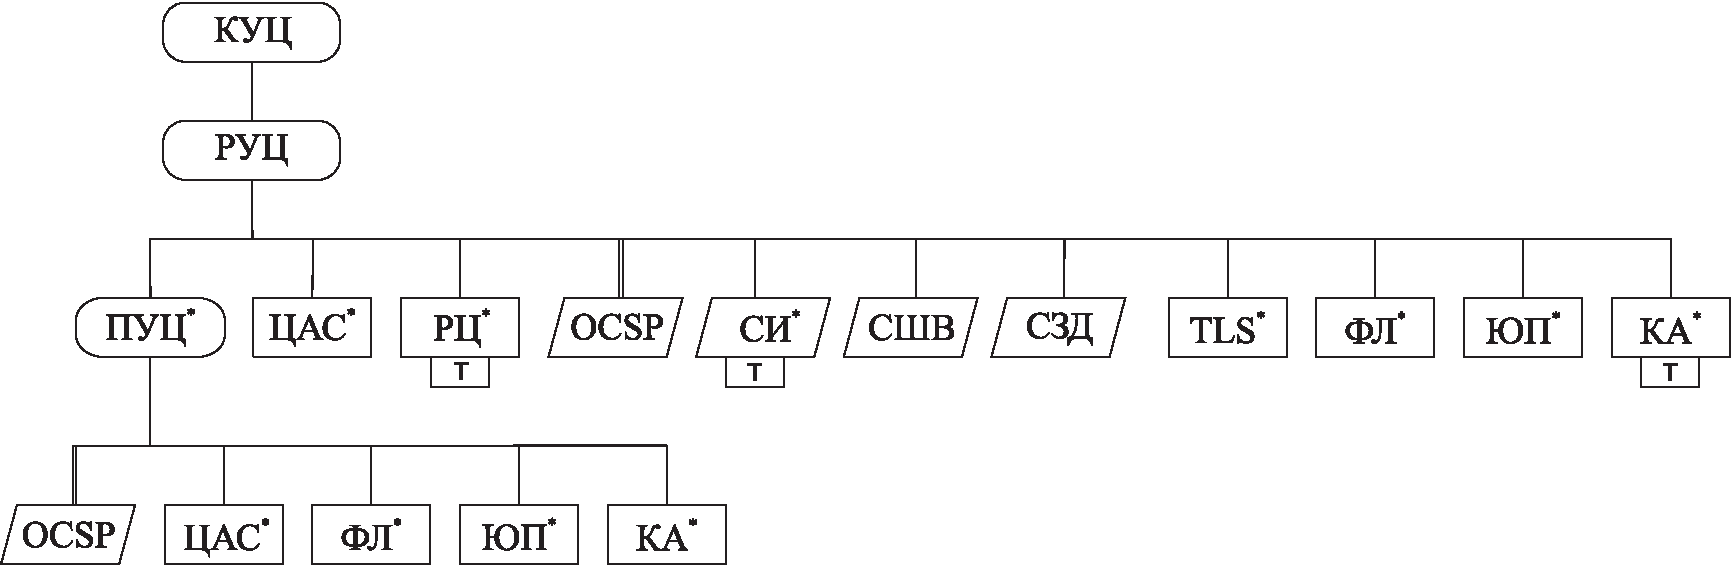
\includegraphics[width=16cm]{../figs/entities}
\end{center}
\caption{Стороны ИОК}
\label{Fig.ENTITIES.1}
\end{figure}

Ролям назначаются идентификаторы АСН.1, определенные в приложении~\ref{ASN1}. 
Идентификаторы имеют вид \verb|{bpki-role n}|,
где \verb|bpki-role|~--- префикс, определенный в приложении,
\texttt{n}~--- числовой код, заданный в таблице~\ref{Table.ENTITIES.Roles}.

\begin{table}[H]
\caption{Роли сторон}
\label{Table.ENTITIES.Roles}
\begin{tabular}{|l|c||l|c|}
\hline
Роль & Код & Роль & Код\\
\hline
\hline
{\bf КУЦ}        & 0    & {\bf СЗД}      & 32 \\
{\bf РУЦ}        & 1    & {\bf СИ}       & 33 \\
{\bf ПУЦ}        & 2    & TLS-сервер     & 50 \\
{\bf ЦАС}        & 10   & ФЛ-резидент    & 60 \\
{\bf РЦ}         & 20   & ФЛ-нерезидент  & 61 \\
{\bf OCSP-сервер}& 30   & ЮП             & 62 \\
{\bf СШВ}        & 31   & КА             & 70 \\
\hline
\end{tabular}
\end{table}

В таблице полужирным шрифтом выделены роли ПУД.
Этим ролям зарезервирован диапазон кодов от~0 до~49.

Операторам ПУД назначаются два идентификатора роли~---
идентификатор ЮП (основной) и идентификатор ПУД. 
%
Агентам ПУД также назначаются два идентификатора: 
идентификатор КА (основной) и идентификатор ПУД. 
%
Дополнительный идентификатор ПУД имеет техническое значение:
оператор сохраняет принадлежность роли ЮП, агент~--- 
роли КА.

Идентификаторы ролей конечных участников указываются в 
расширении~\texttt{CertificatePolicies} их сертификатов
(см.~\ref{FMT.Ext.CP}).
